\section{单换能器激励下超声振幅分布}

超声振动的衰减特性决定了在换能器激励下钢板表面振幅呈现“中心高、四周低”的非均匀分布特征，导致超声振动下不同位置的抗粘减阻效果差异较大，通过优化多换能器的布阵方式可以改善振幅分布特性，从而在肥箱底部钢板表面获得均匀振幅分布。而单换能器振幅分布仿真模型是进行多换能器阵列参数设计与优化的研究基础。为了建立精确的超声波换能器激励钢板的仿真模型，需要对真实的振幅分布进行测量。

\subsection{试验方法}

试验平台如图\ref{pic:振幅分布试验测试平台}所示，该平台主要由超声换能器、超声发生器、试验框架和PSV-400-M2多普勒激光测振仪组成，Q235钢板为厚度为2mm的正方形钢板。由于肥箱底部钢板固定在肥箱子机架四边，为了保证试验及后续仿真的准确性，对钢板进行了四边约束，并将换能器安装在钢板的几何中心。

\begin{figure}[H]
	\centering
	\begin{tikzpicture}
		\node[anchor=south west,inner sep=0] (img) at (0,0) {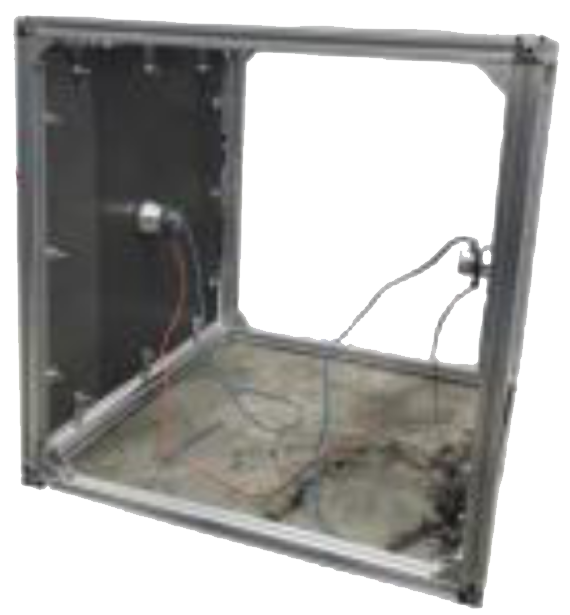
\includegraphics[width=5cm]{../../assets/试验平台.png}};
		% \draw[help lines] (0,0) grid (8,10);
		\draw[thick] (2,1.5) -- (-1,1) node[left]{钢板};
	\end{tikzpicture}
	\caption{振幅分布试验测试平台}
	\label{pic:振幅分布试验测试平台}
\end{figure}

\subsection{用到的测量仪器}

超声振动具有频率高、振幅小的特点，导致测量困难。本试验采用PSV-400-M2多普勒激光测振仪测量单换能器激励下的超声振动振幅分布，可以在不接触被测量物体表面的情况下较远距离对物体表面的振动速度和位移进行测量。该测量方法可以在不需接触被测量物体表面的情况下，通过远距离对物体表面的振动速度和位移进行准确测量，PSV-400-M2多普勒激光测振仪具有0到1MHz的广泛振动频率范围，满足本次实验的要求。测振原理如下：首先，由激光头发射出一束激光（波长$\lambda$），照射到被测量物体表面，反射回来的激光频率会发生变化即多普勒频移（即多普勒频移fD），该频移量与物体的振动速度$v$成正比，根据测量出的多普勒频率，就可以准确计算出被测量表面的振动速度，经过傅里叶变换得出被测钢板表面的振幅。

\begin{figure}[H]
	\centering
	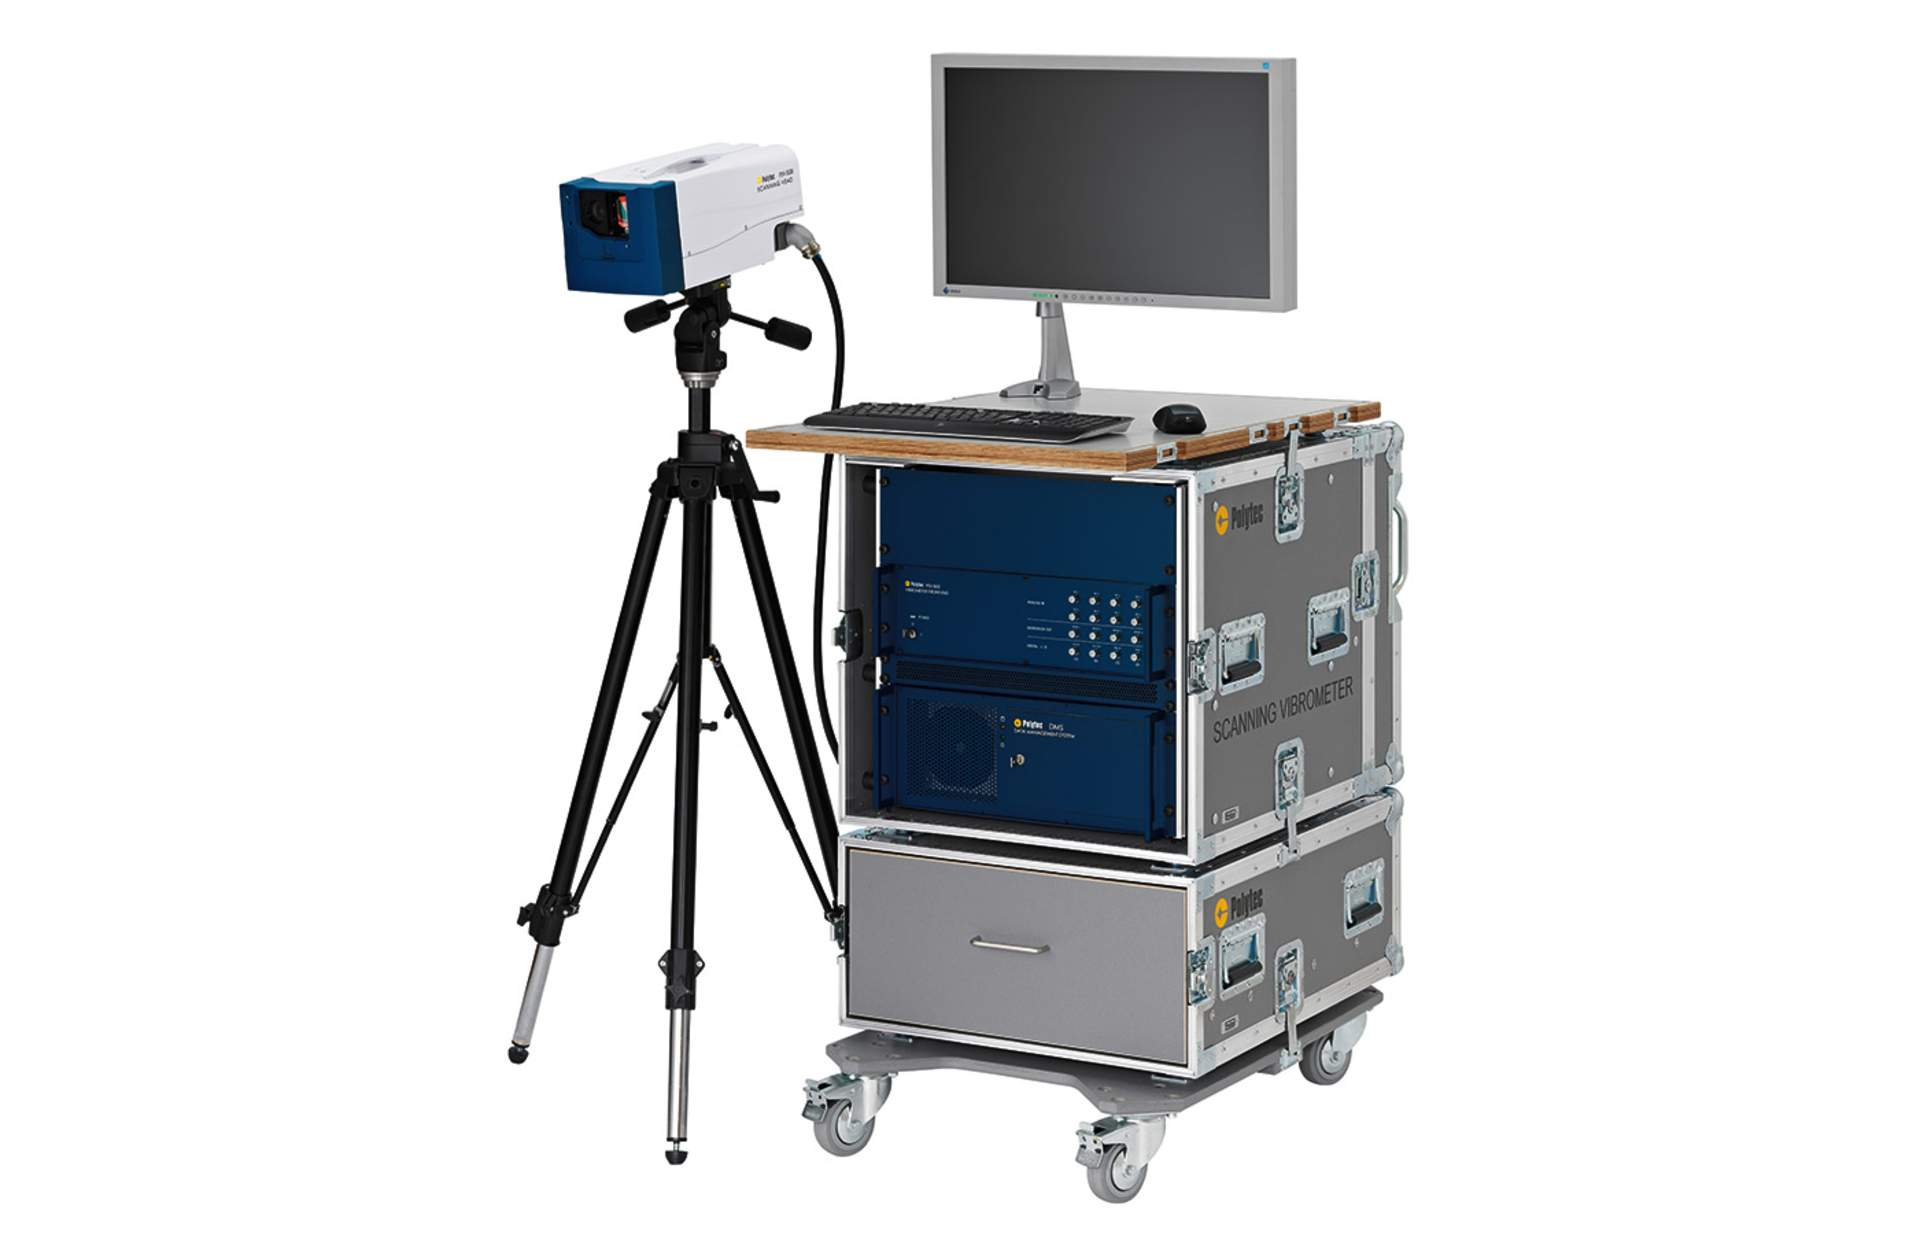
\includegraphics[width=6cm]{../../assets/多普勒激光测振仪.jpg}
	\caption{多普勒激光测振仪}
	\label{pic:多普勒激光测振仪}
\end{figure}